\section{How to Break XML Encryption}

XML Encryption is a W3C standard used for encryption of XML documents~\cite{Eastlake2013}. It is typically used in Web Services applications or for encryption of SAML tokens in Single Sign-On scenarios.

\subsection{Adaptive Chosen-Ciphertext Attacks}

XML Encryption defines (among others) two cryptographic algorithms: RSA PKCS\#1 v1.5 and AES/3DES in CBC (Cipher Block Chaining) mode of operation. These two algorithms are vulnerable to so called adaptive chosen-ciphertext attacks, which has been proven in many practical examples. Thus, it is not surprising that XML Encryption applications were also found to be vulnerable to those attacks:

\begin{itemize}
 \item In 2011, we presented a paper on How to Break XML Encryption~\cite{CCS:JagSom11}, which showed how to attack symmetric key encryption algorithms in CBC mode. The idea is very similar to the typical padding oracle attacks, it is just a slightly more complicated, since we use XML parsing errors as a side-channel. A very good summary on this attack gives Matthew Green.\footnote{\url{http://blog.cryptographyengineering.com/2011/10/attack-of-week-xml-encryption.html}}
 \item In 2012, we showed how to apply Bleichenbacher's attack on the asymmetric encryption algorithm (RSA PKCS\#1) in XML Encryption~\cite{ESORICS:JagSchSom12}. A summary on Bleichenbacher's attack is given on our blog.\footnote{\url{http://web-in-security.blogspot.de/2014/08/old-attacks-on-new-tls-implementations.html}}
\end{itemize}

All you need to know for the WS-Attacker usage is that both attacks belong to the family of adaptive chosen ciphertext attacks.

\begin{figure}[ht]
    \begin{center}
        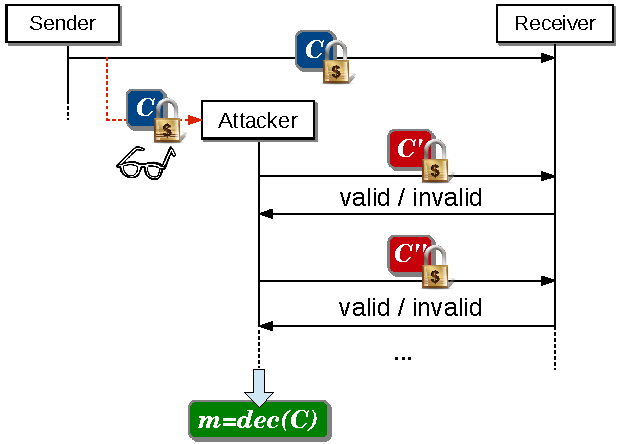
\includegraphics[width=0.5\linewidth]{img/attacker-model-practice2}
    \end{center}
    \caption{Adaptive chosen-ciphertext attack.}
    \label{fig:attacker-model-practice2}
\end{figure}

In an adaptive chosen-ciphertext scenario, the attacker (who eavesdrops an encrypted message) uses the message receiver as an oracle. He sends to the oracle modified ciphertexts and observes its response (it can contain a general error, a parsing failure, or just a valid response text). Based on the responses, he learns the plaintext.


\subsection[XML Signature as a Countermeasure]{XML Signature as a Countermeasure and its Problems}
The attacks are applicable only if the attacker can modify ciphertexts. Integrity of the ciphertexts can be protected using different methods, for example by using XML Signatures. However, this countermeasure brings several problems~\cite{SoSchXMLenc2012}. The first problem is XML Signature Wrapping, as described in \ref{sec:automatic_detection_of_xml_signature_wrapping_attacks}. The second problem is an XML Encryption Wrapping attack. For the description of this attack, consider Figure~\ref{fig:signedEncryptedSoap}, which depicts an encrypted and signed SOAP message.

\begin{figure}[!ht]
    \centering
    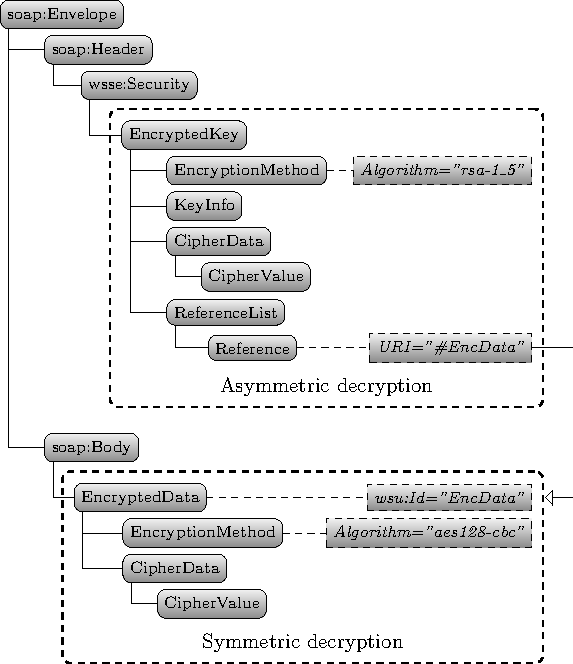
\includegraphics[width=0.55\linewidth]{img/soap_encrypted_signed}
    \caption{Encrypted SOAP message protected by an XML Signature.}
    \label{fig:signedEncryptedSoap}
\end{figure}

The XML Encryption Wrapping attack follows a similar principle as XML Signature Wrapping and enforces the decryption logic to decrypt unauthenticated XML contents. The attacker achieves this by defining new \texttt{EncryptedData} in the SOAP Header element, see Figure~\ref{fig:EncryptionWrapping}.

As can be seen in the figure, the attacker does not move the original SOAP Body element with its content. This enables the Web Service to verify and decrypt the original SOAP Body. However, the Web Service additionally decrypts also a newly defined \texttt{EncryptedData} element with \texttt{Id="oracle"}, since the \texttt{EncryptedKey} element contains a \texttt{DataReference} with \texttt{URI="\#oracle"}. 

\begin{figure}[!ht]
    \centering
    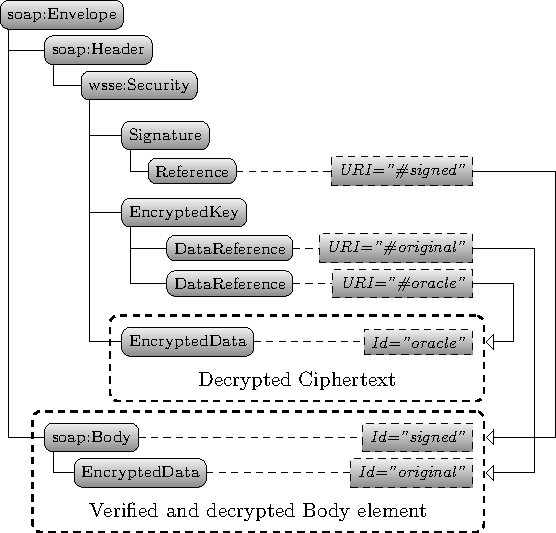
\includegraphics[width=0.55\linewidth]{img/encryption_wrapping}
    \caption{XML Encryption Wrapping attack applied on a signed and encrypted message forces the recipient to process unverified \texttt{EncryptedData}.}
    \label{fig:EncryptionWrapping}
\end{figure}

There are few variations of this attack. It is for example also possible to define a completely new \texttt{EncryptedKey} element with a \texttt{DataReference} \texttt{URI="\#oracle"}. This is applicable to servers processing only one \texttt{EncryptedData} for each \texttt{EncryptedKey} element.


\subsection{Using the XML Encryption Plugin}

A combination of complex cryptographic attacks with XML-specific countermeasures makes it very hard to decide, whether a Web Service is vulnerable to these attacks or not. The XML Encryption plugin allows one to automatically evaluate these attacks. During the test, WS-Attacker sends to the server differently formatted ciphertexts, wrapped using XML Encryption and XML Signature Wrapping techniques. 

In the following, we show how to attack symmetric AES-CBC ciphertexts in Web Services using XML Encryption. For the testing purposes, we configured an IBM Datapower Web Service, which simply decrypts a ciphertext and responds with a test message in a case the decryption was valid. Further prerequisite for the attack is a valid WSDL file (or a valid Web Service endpoint) and a SOAP message containing encrypted content.

To execute the attack, we first start WS-Attacker and load the WSDL file. 
Afterwards, we send a test request (our SOAP message containing the encrypted content) to the Web Service. The test request initializes WS-Attacker and the contained plugins: WS-Attacker automatically analyzes whether the message contains encrypted content and whether it is possible to execute an attack on XML Encryption.

\begin{figure}[!ht]
    \centering
    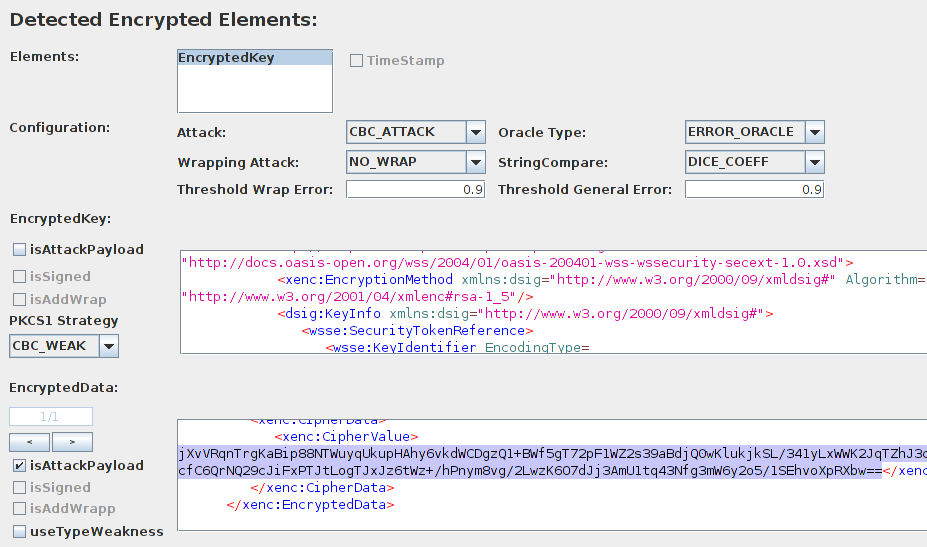
\includegraphics[width=0.95\linewidth]{img/xenc-config1}
    \caption{XML Encryption attack configuration.}
    \label{fig:xenc-config1}
\end{figure}

After initializing WS-Attacker with the test request, we can move to Plugin configuration. We choose XML Encryption attack, which contains the following configuration (see Figure~\ref{fig:xenc-config1}). Here are the relevant parts and their description:

 \begin{itemize}
  \item Elements: list of \texttt{EncryptedKey} elements contained in this message. In our case, this message contains only one \texttt{EncryptedKey} element, but there are more complicated scenarios, where messages include more ciphertexts. This option allows us then to choose, which of the encrypted elements is going to be attacked.
  \item Attack: we can choose between CBC and PKCS\#1 attack. Now, we work with the CBC attacks.
  \item Wrapping attack: If the message contains an XML Signature to protect message authenticity, we can automatically adapt Wrapping attacks to overcome the authenticity check. In the tested message, there is no XML Signature so we use \texttt{NO\_WRAP}.
  \item String Compare: In order to apply oracle attacks, we have to map real server responses to "oracle" responses. Real responses can however contain timestamps and message ids, which can make the mapping complicated. String comparison methods allow us to define thresholds for message similarities. This makes mapping much easier. We typically use the default Dice-coefficient method with a threshold 0.9.
 \end{itemize}

After setting the above options, we have to select the attack payload (the CBC ciphertext) using the check box located on the right side. 

Now, we are ready to configure the oracle in the Server Error Table configuration. Here, we click on "New Messages", which sends a few hundreds of messages to the server. Afterwards, we have to provide a mapping from real messages to oracle results. Since we set the Dice-coefficient with a 0.9 threshold, we received only two messages. In the next figure, you can see we configured the server response with an \texttt{EncryptedData} element to be an INVALID oracle response. This is because IBM Datapower with our configuration is not able to decrypt the request and just mirrors the request.\footnote{To configure your oracle correctly, you have to know the server behavior and decide, whether an error comes from message parsing, message decryption, or from a different module.}

\begin{figure}[!ht]
    \centering
    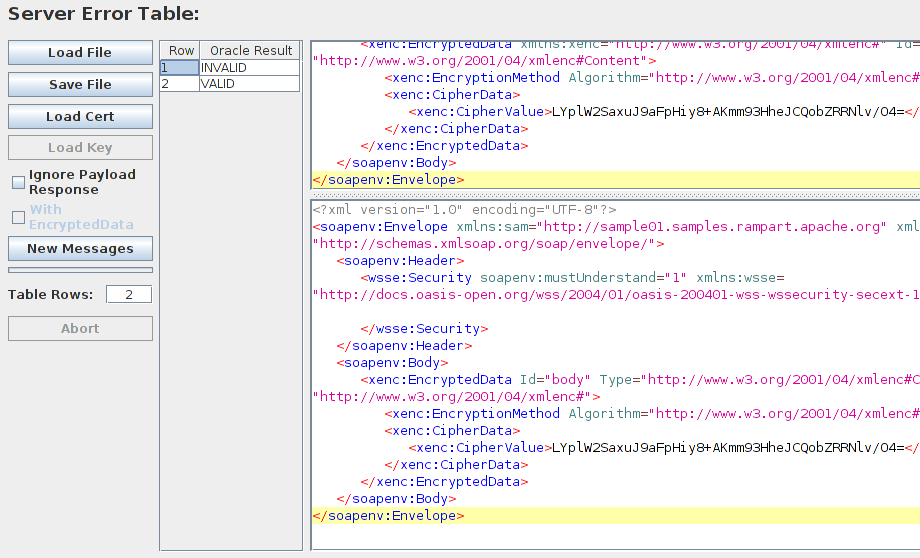
\includegraphics[width=0.95\linewidth]{img/xenc-config2}
    \caption{Configuring XML Encryption server oracle with valid and invalid responses.}
    \label{fig:xenc-config2}
\end{figure}

Finally, we configured WS-Attacker and we can start the attack. After few minutes and about 4900 server queries, we can see that we could successfully decrypt 221 message bytes (including the comments and namespaces).

\begin{figure}[!ht]
    \centering
    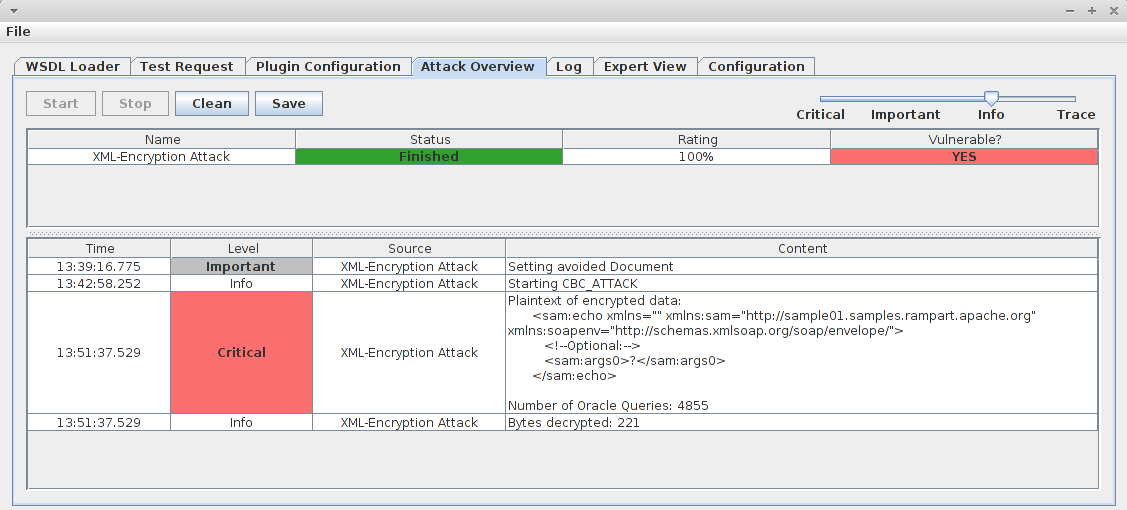
\includegraphics[width=\linewidth]{img/xenc-result}
    \caption{Result of the XML Encryption attack shows the decrypted content.}
    \label{fig:xenc-result}
\end{figure}
